\section{Active Appearance Models}
\label{sec:aam}

\begin{figure*}
	\centering
	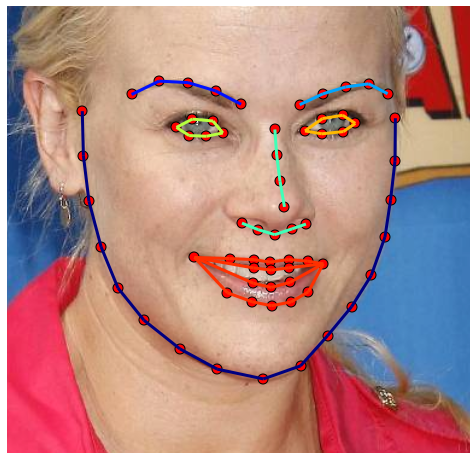
\includegraphics[width=0.16\textwidth]{figures/img0.png}
	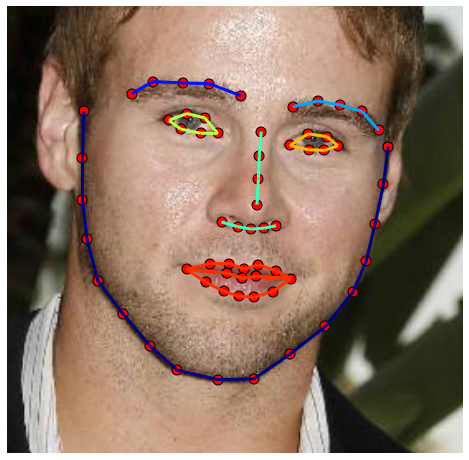
\includegraphics[width=0.16\textwidth]{figures/img1.png}
	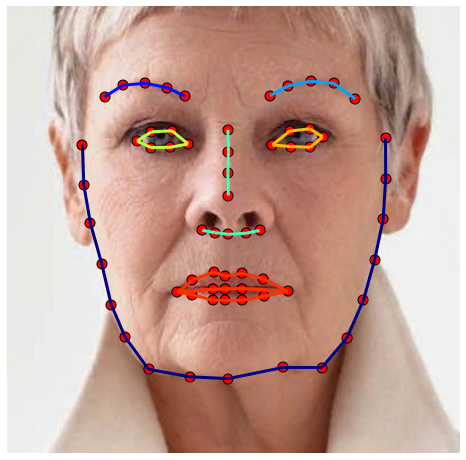
\includegraphics[width=0.16\textwidth]{figures/img2.png}
	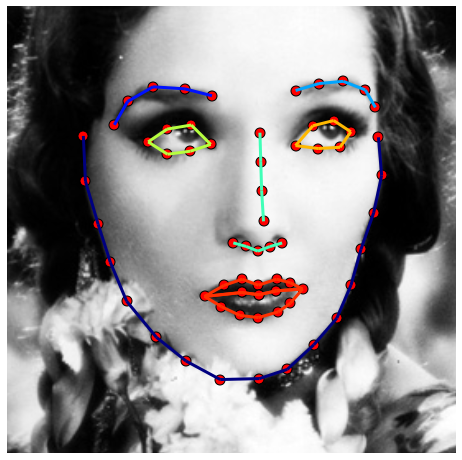
\includegraphics[width=0.16\textwidth]{figures/img3.png}
	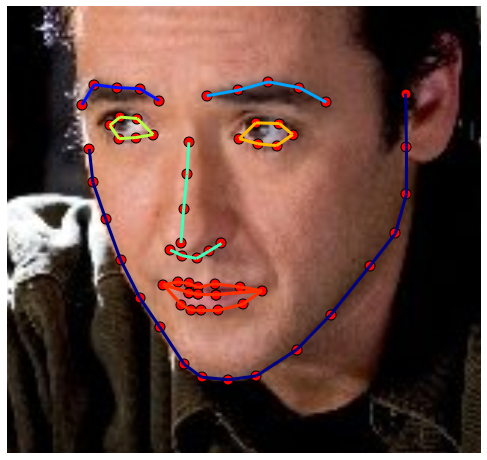
\includegraphics[width=0.16\textwidth]{figures/img4.png}
	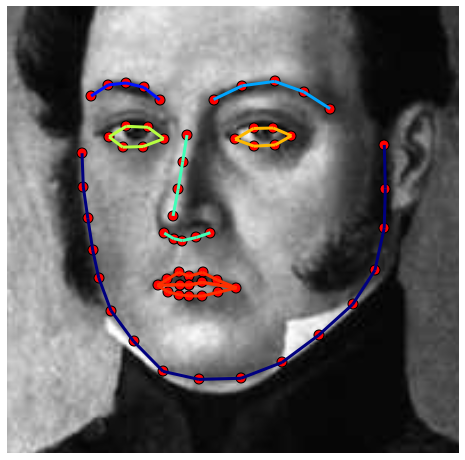
\includegraphics[width=0.16\textwidth]{figures/img5.png}
	\caption{Exemplar images from the Labeled Faces in-the-Wild (LFPW) dataset \cite{Belhumeur2011} for which a consistent set of sparse landmarks representing the shape of the object being model (human face) has been manually defined.}
	\label{fig:afw_exp}
\end{figure*}

Active Appearance Models (AAMs) \cite{Cootes2001,Matthews2004} are generative parametric models that explain visual variations, in terms of shape and appearance, within a particular object class. AAMs are built from a collection of images for which the spatial position of a sparse set of landmark points $\mathbf{x}_i = (x_i, y_i)^T \in \mathcal{R}^2$ representing the shape $\mathbf{s} = (x_1, y_1, \dots, x_v, y_v)^T \in \mathcal{R}^{2v \times 1}$ of the object being modeled has been manually defined a priori. 

AAMs are themselves composed of three different models:
\begin{inparaenum}[(i)]
	\item shape model; 
	\item appearance model; and
	\item motion model. 
\end{inparaenum} 

The shape model, which is also referred to as Point Distribution Model (PDM), is obtained by typically applying Principal Component Analysis (PCA) to the set of object's shapes defined by the previous landmarks points. The resulting shape model is mathematically expressed as:
\begin{equation}
	\begin{aligned}
		\mathbf{s} & = \mathbf{\bar{s}} + \sum_{i=1}^n p_i \mathbf{s}_i 
        \\
        & = \mathbf{\bar{s}} + \mathbf{S} \mathbf{p}
	\end{aligned}
\end{equation}
where $\mathbf{\bar{s}} \in \mathcal{R}^{2v \times 1}$ is mean shape, and $\mathbf{S} \in  \mathcal{R}^{2v \times  n}$ and $\mathbf{p} \in \mathcal{R}^{n \times 1}$ denote the shape bases and shape parameters, respectively. In order to allow a particular shape instance $\mathbf{s}$ to be arbitrarily positioned in space, the previous model can be augmented with a global similarity transform. Note that this normally requires the initial shapes to be normalized with respect to the same type of transform (typically using Procrustes Analysis (PA)) before PCA is applied. This result in the following expression for each landmark point of the shape model is:
\begin{equation}
	\begin{aligned}
		\mathbf{x}_i & = s \mathbf{R} \left( \mathbf{\bar{x}}_i + \mathbf{X}_i \mathbf{p} \right) + \mathbf{t}
	\end{aligned}
\end{equation}
where $s$, $\mathbf{R} \in \mathcal{R}^{2 \times 2}$ and $\mathbf{t} \in \mathcal{R}^2$  denote the scale, rotation and translation applied by the global similarity transform, respectively. Using the orthonormalization procedure descrived in \cite{Matthews2004} the final expression for the shape model can be compactly written as the linear combination of a set of bases:
\begin{equation}
	\begin{aligned}
		\mathbf{s} & = \mathbf{\bar{s}} + \sum_{i=1}^4 p^*_i \mathbf{s}^*_i + \sum_{i=1}^n p_i \mathbf{s}_i 
        \\
        & = \mathbf{\bar{s}} + \mathbf{S} \mathbf{p}
	\end{aligned}
    \label{eq:shape_model}
\end{equation}
where $\mathbf{S} = (\mathbf{s}^*_1, \dots, \mathbf{s}^*_4, \mathbf{s}_1, \cdots, \mathbf{s}_n) \in \mathcal{R}^{2v \times (n+4)}$ and $\mathbf{p} = (p^*_1, \dots, p^*_4, p_1, \dots, p_n)^T \in \mathcal{R}^{(n+4) \times 1}$ are redefined as the concatenation of the similarity bases $\mathbf{s}^*_i$ and similarity parameters $p^*_i$ with the original $\mathbf{S}$ and $\mathbf{p}$, respectively.

The appearance model is obtained by warping the original images onto a common reference frame (typically defined in terms of the mean shape $\mathbf{\bar{s}}$) and applying PCA to the obtained warped images. Mathematically, the appearance model is defined by the following expression:
\begin{equation}
	\begin{aligned}
		A(\mathbf{x}) & = \bar{A}(\mathbf{x}) + \sum_{i=1}^m c_i A_i(\mathbf{x})
	\end{aligned}
    \label{eq:app_model}
\end{equation}
where $\mathbf{x} \in \Omega$ denote all pixels positions on the reference frame, and $\bar{A}(\mathbf{x})$, $A_i(\mathbf{x})$ and $c_i$ denote the mean texture, the appearance bases and appearance parameters, respectively. Denoting $\mathbf{a} = \text{vec}(A(\mathbf{x}))$ as the vectorized version of the previous appearance instance, equation \ref{eq:app_model} can be concisely written in vector form as
\begin{equation}
	\begin{aligned}
		\mathbf{a} & = \mathbf{\bar{a}} + \mathbf{A} \mathbf{c}
	\end{aligned}
    \label{eq:app_model_vec}
\end{equation}
where $\mathbf{a} \in \mathcal{R}^{F \times 1}$ is the mean appearance, and $\mathbf{A} \in  \mathcal{R}^{F \times  m}$ and $\mathbf{c} \in \mathcal{R}^{m \times 1}$ denote the appearance bases and appearance parameters, respectively.

The role of the motion model, denoted by $\mathcal{W}(\mathbf{x}; \mathbf{p})$, is to extrapolate the position of all pixel positions $\mathbf{x} \in \Omega$ from the reference frame to a particular shape instance $\mathbf{s}$ (and vice-versa) based on their relative position with respect to the sparse set of landmarks defining the shape model (for which direct correspondences are always known). Classic motion models for AAMs are Piece Wise Affine (PWA) \cite{Cootes2004,Matthews2004} and Thin Plate Splines (TPS) \cite{Cootes2004,Papandreou2008} warps. 

Given an image $I(\mathbf{x})$ containing the object of interest, its manually annotated ground truth shape $\mathbf{s}$, and a particular motion model $\mathcal{W}(\mathbf{x}, \mathbf{p})$; the two main assumptions behind AAMs are:

\begin{enumerate}
	\item The ground truth shape of the object can be well approximated by the shape model
	\begin{eqnarray}
		\begin{aligned}
			\mathbf{s} & \approx \mathbf{\bar{s}} + \mathbf{S} \mathbf{p}
		\end{aligned}
	    \label{eq:aam_1}
	\end{eqnarray}

	\item The object's appearance can be well approximated by the appearance model after the image is warped, using the motion model and the the previous shape approximation, onto the reference frame
	\begin{eqnarray}
		\begin{aligned}
			\mathbf{i}[\mathbf{p}] & \approx \mathbf{\bar{a}} + \mathbf{A} \mathbf{c} 
		\end{aligned}
	    \label{eq:aam_2}
	\end{eqnarray}
	where $\mathbf{i}[\mathbf{p}] = \mathrm{vec}(I(\mathcal{W}(\mathbf{x}; \mathbf{p})))$ denotes the vectorized version of the warped image. Note that, the warp $\mathcal{W}(\mathbf{x}; \mathbf{p}))$ which explicitly depends on the shape parameters $\mathbf{p}$, relates the previous shape and appearance models and it is a central part of the AAMs formulation
\end{enumerate}

Because of their explicit use of the motion model, the two previous assumptions provide a concise and unambiguous way to define AAMs. These assumption will be used in next section \ref{sec:paam} to introduce a more general and probabilistic formulation of AAMs. At this point, it is worth to mention that the vector notation of equations \ref{eq:aam_1} and \ref{eq:aam_2} will be, in general, the preferred notation in this paper.

